\chapter{Compass and Straightedge Constructions}
\begin{quote} 
\begin{tabular}{rl}
\textit{Mephistopheles:} & I must say there is an obstacle \\
                         & That prevents my leaving:\\
                         & It's the pentagram on your threshold.\\
\textit{Faust:}          & The pentagram impedes you? \\
                         & Tell me then, you son of hell,\\
                         & If this stops you, how did you come in?\\
\textit{Mephistopheles:} & Observe! The lines are poorly drawn;\\
                         & That one, the outer angle, \\
                         & Is open, the lines don't meet.
\end{tabular}

\hfill---G\"othe, \textit{Faust} act I, scene III
\end{quote}

\section{Constructions}

About a century before the time of \index{Euclid}Euclid,
\index{Plato}Plato---a student of \index{Socrates}Socrates---declared
that the compass and straightedge should be the only tools of the
geometer. Why would he do such a thing? For one thing, both the the
compass and straightedge are fairly simple instruments. One draws
circles, the other draws lines---what else could possibly be needed to
study geometry? Moreover, rulers and protractors are far more complex
in comparison and people back then couldn't just walk to the campus
bookstore and buy whatever they wanted. However, there are other
reasons:
\begin{enumerate}        
\item Compass and straightedge constructions are \textbf{independent
  of units}.
\item Compass and straightedge constructions are \textbf{theoretically
  correct}.
\item Combined, the compass and straightedge seem like
  \textbf{powerful tools}.
\end{enumerate}



\paragraph{Compass and straightedge constructions are \textbf{independent of units}.} 
Whether you are working in centimeters or miles, compass and
straightedge constructions work just as well. By not being locked to
set of units, the constructions given by a compass and straightedge
have certain generality that is appreciated even today.


\paragraph{Compass and straightedge constructions are \textbf{theoretically correct}.} 
In mathematics, a correct method to solve a problem is more valuable
than a correct solution. In this sense, the compass and straightedge
are ideal tools for the mathematician. Easy enough to use that the
rough drawings that they produce can be somewhat relied upon, yet
simple enough that the tools themselves can be described
theoretically. Hence it is usually not too difficult to connect a
given construction to a formal proof showing that the construction is
correct.


\paragraph{Combined, the compass and straightedge seem like \textbf{powerful tools}.} 
No tool is useful unless it can solve a lot of problems. Without a
doubt, the compass and straightedge combined form a powerful
tool. Using a compass and straightedge, we are able to solve many
problems exactly. Of the problems that we cannot solve exactly, we can
always produce an approximate solution.





\index{constructions|see{compass and straightedge \textit{or}
    origami}} We'll start by giving the rules of compass and
straightedge constructions:

\subsubsection*{Rules for Compass and Straightedge Constructions}
\begin{enumerate}
\item You may only use a compass and straightedge.
\item You must have two points to draw a line.
\item You must have a point and a line segment to draw a circle. The
  point is the center and the line segment gives the radius.
\item Points can only be placed in two ways:
\begin{enumerate}
\item As the intersection of lines and/or circles.
\item As a \textbf{free point}\index{free point}, meaning the location
  of the point is not important for the final outcome of the
  construction.
\end{enumerate}
\end{enumerate}

Our first construction is also Euclid's first construction:

\begin{construction}[Equilateral Triangle]\index{compass and straightedge!equilateral triangle} We wish to construct an equilateral triangle given the length of one 
side.
\begin{enumerate} 
\item Open your compass to the width of the line segment.
\item Draw two circles, one with the center being each end point 
of the line segment.
\item The two circles intersect at two points.  Choose one and 
connect it to both of the line segment's endpoints.
\end{enumerate}
\[
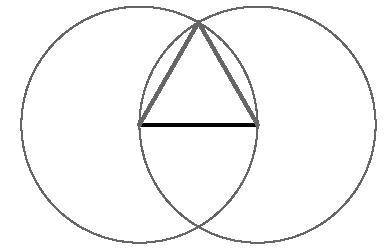
\includegraphics[scale=0.9]{../graphics/eqtri.pdf}
\]
\end{construction}

Euclid's second construction will also be our second construction:

\begin{construction}[Transferring a Segment]\index{compass and straightedge!transferring a segment}
Given a segment, we wish to move it so that it starts on a given
point, on a given line.
\begin{enumerate}        
\item Draw a line through the point in question.
\item Open your compass to the length of the line segment and draw a circle with the given point as its center.
\item The line segment consisting of the given point and the intersection of the circle and the line 
is the transferred segment.
\end{enumerate}
\end{construction}

If you read \emph{The Elements}, you'll see that Euclid's construction is
much more complicated than ours.   Apparently, Euclid felt the need to
justify the ability to move a distance. Many sources say that Euclid
used what is called a \index{compass!collapsing}\index{collapsing
compass}\textit{collapsing compass}, that is a compass that collapsed
when it was picked up. However, I do not believe that such an
invention ever existed. Rather this is something that lives in the
conservative geometer's head.


Regardless of whether the difficulty of transferring distances was theoretical
or physical, we need not worry when we do it.  In fact, Euclid's
proof of the above theorem proves that our modern way of using the
compass to transfer distances is equivalent to using the so-called
collapsing compass.

\begin{question} Exactly how would one prove that the modern compass is equivalent 
to the collapsing compass? Hint: See Euclid's proof.
\end{question}
\QM


\begin{construction}[Bisecting a Segment]\index{compass and straightedge!bisecting a segment} 
Given a segment, we wish to cut it in half.
\begin{enumerate}
\item Open your compass to the width of the segment.
\item Draw two circles, one with the center being at each end point 
of the line segment.
\item The circles intersect at two points.  Draw a line through 
these two points.
\item The new line bisects the original line segment.
\end{enumerate}
\[
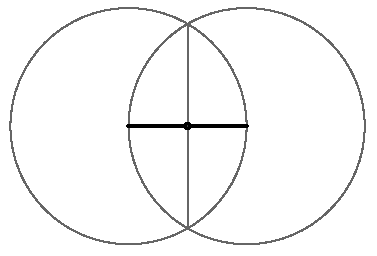
\includegraphics[scale=0.9]{../graphics/bisectseg.pdf}
\]
\end{construction}

\begin{construction}[Perpendicular to a Line through a Point]\index{compass and straightedge!perpendicular to a line through a point}  
Given a point and a line, we wish to construct a line perpendicular to
the original line that passes through the given point.
\begin{enumerate}
\item Draw a circle centered at the point large enough  
       to intersect the line in two distinct points.
\item Bisect the line segment. The line used to do this 
       will be the desired line.
\end{enumerate}
\[
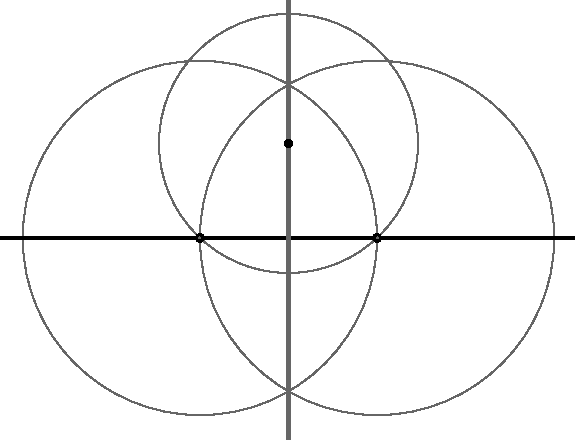
\includegraphics[scale=0.8]{../graphics/perpfrompoint.pdf}
\]
\end{construction}





\begin{construction}[Bisecting an Angle]\index{compass and straightedge!bisecting an angle} 
We wish to divide an angle in half.
\begin{enumerate}
\item Draw a circle with its center being the vertex of the 
angle.
\item Draw a line segment where the circle intersects the lines.
\item Bisect the new line segment.  The bisector will bisect the angle.
\end{enumerate}
\[
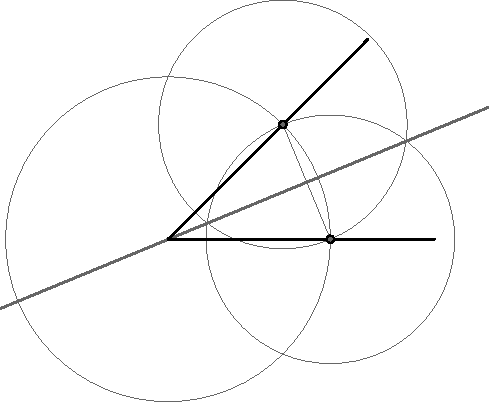
\includegraphics{../graphics/bisectangle.pdf}
\]
\end{construction}


We now come to a very important construction:

\begin{construction}[Copying an Angle]\index{compass and straightedge!copying an angle} 
Given a point on a line and some angle, we wish to copy the 
given angle so that the new angle has the point as its 
vertex and the line as one of its edges.
\begin{enumerate}
\item Open the compass to a fixed width and make a circle 
centered at the vertex of the angle.
\item Make a circle of the same radius on the line with the point.
\item Open the compass so that one end touches the $1$st circle 
where it hits an edge of the original angle, with the other end of the compass extended to where the $1$st circle hits the other edge of the original angle.
\item Draw a circle with the radius found above with its center 
where the second circle hits the line.
\item Connect the point to where the circles meet. This is the other leg of the angle we are constructing.
\end{enumerate}
\[
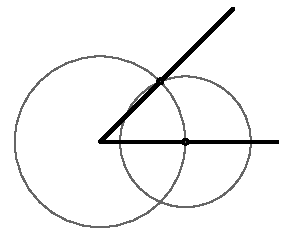
\includegraphics{../graphics/copyangle.pdf}
\]
\end{construction}



\begin{construction}[Parallel to a Line through a Point]\index{compass and straightedge!parallel to a line through a point} 
 Given a line and a point, we wish to construct another line parallel
 to the first that passes through the given point.
\begin{enumerate}
\item Draw a circle around the given point that passes through the given line at two points.
\item We now have an isosceles triangle, duplicate this triangle.
\item Connect the top vertexes of the triangles and we get a parallel line.
\end{enumerate}
\vspace{1cm}
\[
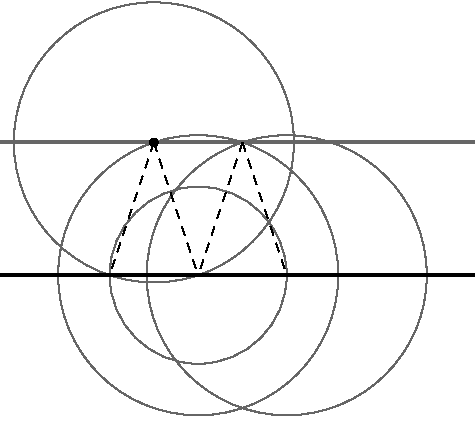
\includegraphics[scale=0.9]{../graphics/parallel.pdf}
\]
\end{construction}


\begin{question} Can you give another different construction?
\end{question}
\QM


\begin{problems}
\begin{enumerate}
\item What are the rules for compass and straightedge constructions?
\item What is a collapsing compass? Why don't we use them or worry about them any more?
\item Prove that the collapsing compass is equivalent to the modern compass.
\item Given a line segment, construct an equilateral triangle whose edge has the length of the given segment. Explain the steps in your construction.
\item Use a compass and straightedge to bisect a given line segment. Explain the steps in your construction.
\item Given a line segment with a point on it, construct a line perpendicular to the segment that passes through the given point. Explain the steps in your construction.
\item Use a compass and straightedge to bisect a given angle. Explain the steps in your construction.
\item Given an angle and some point, use a compass and straightedge to copy the angle so that the new angle has as its vertex the given point. Explain the steps in your construction.
\item Given a point and line, construct a line perpendicular to the given line that passes through the given point. Explain the steps in your construction.
\item Given a point and line, construct a line parallel to the given line that passes through the given point. Explain the steps in your construction.
\item Given a length of $1$, construct a triangle whose perimeter is a
  multiple of $6$. Explain the steps in your construction.
\item Construct a $30$-$60$-$90$ right triangle. Explain the steps in your
  construction.
\item Given a length of $1$, construct a triangle with a perimeter of
  $3 + \sqrt{5}$. Explain the steps in your construction.\fixnote{For all problems, How do you know it works?}
\item Given a length of $1$, construct a triangle with a perimeter that is a multiple of
  $2 + \sqrt{2}$. Explain the steps in your construction.
\item Here is a circle and here is the side length of an inscribed
  regular $5$-gon.
\[
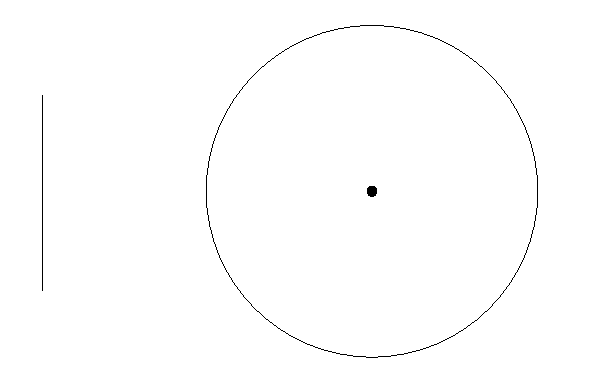
\includegraphics{../graphics/5gonPiece.pdf}
\]
Construct the regular $5$-gon. Explain the steps in your construction.
\item Here is a piece of a regular $7$-gon.
\[
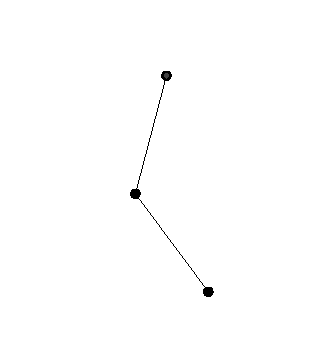
\includegraphics{../graphics/7gonPiece.pdf}
\]
Construct the entire regular $7$-gon. Explain the steps in your
construction.
\end{enumerate}
\end{problems}

\newpage



\section{Anatomy of Figures}


In studying geometry we seek to discover the points that can be
obtained given a set of rules. In our case the set of rules consists
of the rules for compass and straightedge constructions.

\begin{question} 
In regards to compass and straightedge constructions, what is a
\textit{point}?
\end{question}
\QM

\begin{question}
In regards to compass and straightedge constructions, what is a
\textit{line}?
\end{question}
\QM


\begin{question}
In regards to compass and straightedge constructions, what is a
\textit{circle}?
\end{question}
\QM


OK, those are our basic figures, pretty easy right? Now I'm going to
quiz you about them:

\begin{question} 
Place two points randomly in the plane. Do you expect to be able to
draw a single line that connects them?
\end{question}
\QM

\begin{question} 
Place three points randomly in the plane. Do you expect to be able to
draw a single line that connects them?
\end{question}
\QM

\begin{question} 
Place two lines randomly in the plane. How many points do you expect
them to share?
\end{question}
\QM


\begin{question} 
Place three lines randomly in the plane. How many points do you expect
all three lines to share?
\end{question}
\QM


\begin{question} 
Place three points randomly in the plane. Will you (almost!) always be
able to draw a circle containing these points? If no, why not? If yes,
how do you know?
\end{question}
\QM




\subsection{Lines Related to Triangles}

Believe it or not, in mathematics we often try to study the simplest
objects as deeply as possible. After the objects listed above,
triangles are among the most basic of geometric figures, yet there is
much to know about them.  There are several lines that are commonly
associated to triangles. Here they are:
\begin{itemize}
\item Perpendicular bisectors of the sides.
\item Bisectors of the angles.
\item Altitudes of the triangle.
\item Medians of the triangle. 
\end{itemize}

The first two lines above are self-explanatory. The next two need definitions.

\begin{definition}\index{altitude} 
An \textbf{altitude} of a triangle is a line segment originating at a
vertex of the triangle that meets the line containing the opposite
side at a right angle.
\end{definition}


\begin{definition}\index{median} 
A \textbf{median} of a triangle is a line segment that connects a
vertex to the midpoint of the opposite side.
\end{definition}

\begin{question} 
The intersection of any two lines containing the altitudes of a
triangle is called an \textbf{orthocenter}\index{orthocenter}. How
many orthocenters does a given triangle have?
\end{question}
\QM


\begin{question} 
The intersection of any two medians of a triangle is called a
\textbf{centroid}\index{centroid}. How many centroids does a given
triangle have?
\end{question}
\QM


\begin{question} What is the physical meaning of a centroid?
\end{question}
\QM




\subsection{Circles Related to Triangles}


There are also two circles that are commonly associated to
triangles. Here they are:
\begin{itemize}
\item The circumcircle.
\item The incircle.
\end{itemize}

These aren't too bad. Check out the definitions.

\begin{definition}\index{circumcircle}\index{circumcenter}
The \textbf{circumcircle} of a triangle is the circle that contains
all three vertexes of the triangle. Its center is called the
\textbf{circumcenter} of the triangle.
\[
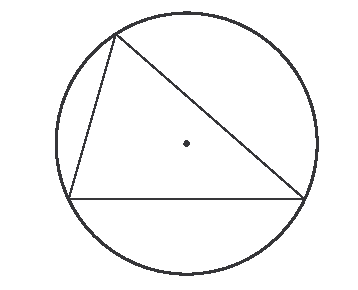
\includegraphics[width=2in]{../graphics/circumcircle.pdf}
\]
\end{definition}

\begin{question} Does every triangle have a circumcircle?
\end{question}
\QM

\begin{definition}\index{incircle}\index{incenter}
The \textbf{incircle} of a triangle is the largest circle that will
fit inside the triangle. Its center is called the \textbf{incenter} of
the triangle.
\[
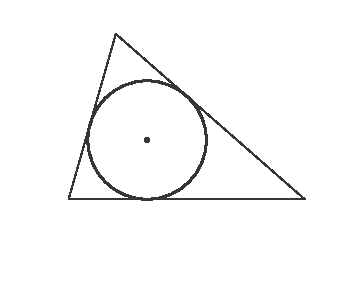
\includegraphics[width=2in]{../graphics/incircle.pdf}
\]
\end{definition}


\begin{question} Does every triangle have an incircle?
\end{question}
\QM


\begin{question} 
Are any of the lines described above related to these circles and/or
centers? Clearly articulate your thoughts.
\end{question}
\QM


\begin{problems}
\begin{enumerate}
\item Compare and contrast the idea of ``intersecting sets'' with the
  idea of ``intersecting lines.''
\item Place three points in the plane. Give a detailed discussion
  explaining how they may or may not be on a line.
\item Place three lines in the plane. Give a detailed discussion explaining
  how they may or may not intersect.
\item Explain how a perpendicular bisector is different from an
  altitude. Draw an example to illustrate the difference.
\item Explain how a median is different from an angle bisector.  Draw an
  example to illustrate the difference.
\item What is the name of the point that is the same distance from all
  three sides of a triangle? Explain your reasoning.
\item What is the name of the point that is the same distance from all
  three vertexes of a triangle? Explain your reasoning.
\item Could the circumcenter be outside the triangle? If so, draw a
  picture and explain. If not, explain why not using pictures as
  necessary.
\item Could the orthocenter be outside the triangle? If so, draw a
  picture and explain. If not, explain why not using pictures as
  necessary.
\item Could the incenter be outside the triangle? If so, draw a
  picture and explain. If not, explain why not using pictures as
  necessary.
\item Could the centroid be outside the triangle? If so, draw a
  picture and explain. If not, explain why not using pictures as
  necessary.
\item Are there shapes that do not contain their centroid? If so, draw
  a picture and explain. If not, explain why not using pictures as
  necessary.
\item Draw an equilateral triangle. Now draw the lines containing the
  altitudes of this triangle. How many orthocenters do you have as
  intersections of lines in your drawing? Hints:
\begin{enumerate}
\item More than one.
\item How many triangles are in the picture you drew?
\end{enumerate}
\item Given a triangle, construct the circumcenter. Explain the steps
  in your construction.\index{circumcenter}
\item Given a triangle, construct the orthocenter. Explain the steps
  in your construction.\index{orthocenter}
\item Given a triangle, construct the incenter. Explain the steps in
  your construction.\index{incenter}
\item Given a triangle, construct the centroid. Explain the steps in
  your construction.\index{centroid}
\item Given a triangle, construct the incircle. Explain the steps in
  your construction.\index{incircle}
\item Given a triangle, construct the circumcircle. Explain the steps
  in your construction.\index{circumcircle}
\item Given a circle, give a construction that finds its center. 
\item Where is the circumcenter of a right triangle? Explain your
  reasoning.
\item Where is the orthocenter of a right triangle? Explain your
  reasoning.
\item Can you draw a triangle where the circumcenter, orthocenter,
  incenter, and centroid are all the same point?  If so, draw a
  picture and explain. If not, explain why not using pictures as
  necessary.
\item True or False: Explain your conclusions.
\begin{enumerate}
\item An altitude of a triangle is always perpendicular to a line
  containing some side of the triangle.
\item An altitude of a triangle always bisects some side of the
  triangle.
\item The incenter is always inside the triangle.
\item The circumcenter, the centroid, and the orthocenter always lie in a line.
\item The circumcenter can be outside the triangle.
\item The orthocenter is always inside the triangle.
\item The centroid is always inside the incircle.
\end{enumerate}
\item Given 3 distinct points not all in a line, construct a circle
  that passes through all three points. Explain the steps in your
  construction.
\end{enumerate}
\end{problems}

\newpage

\section{Trickier Constructions}

\begin{question} 
How do you construct regular polygons? In particular, how do you
construct regular: $3$-gons, $4$-gons, $5$-gons, $6$-gons, $7$-gons,
$8$-gons, $10$-gons, $12$-gons, $17$-gons, $24$-gons, and $144$-gons?
\end{question}
\QM

Well the equilateral triangle is easy. It was the first construction
that we did. What about squares? What about regular hexagons? It turns
out that they aren't too difficult. What about pentagons? Or say
$n$-gons? We'll have to think about that. Let's leave the difficult
land of $n$-gons and go back to thinking about nice, three-sided
triangles.

\begin{construction}[SAS Triangle]\index{compass and straightedge!SAS triangle}  
Given two sides with an angle between them, we wish to construct the
triangle with that angle and two adjacent sides.
\begin{enumerate}
\item Transfer the one side so that it starts at the vertex of the
  angle.
\item Transfer the other side so that it starts at the vertex. 
\item Connect the end points of all moved line segments.
\end{enumerate}
\end{construction}

The ``SAS'' in this construction's name spawns from the fact that it
requires two sides with an angle \textit{between} them. The SAS
Theorem states that we can obtain a unique triangle given two sides
and the angle between them.


\begin{construction}[SSS Triangle]\index{compass and straightedge!SSS triangle} 
Given three line segments we wish to construct the triangle that has
those three sides if it exists.
\begin{enumerate}
\item Choose a side and select one of its endpoints.
\item Draw a circle of radius equal to the length of the second side
  around the chosen endpoint.
\item Draw a circle of radius equal to the length of the third side
  around the other endpoint.
\item Connect the end points of the first side and the intersection of
  the circles. This is the desired triangle.
\end{enumerate}
\end{construction}


\begin{question} 
Can this construction fail to produce a triangle? If so, show how. If
not, why not?
\end{question}
\QM

\begin{question}
Remember earlier when we asked about the converse to the Pythagorean
Theorem?\index{Pythagorean Theorem} Can you use the construction above
to prove the converse of the Pythagorean Theorem?
\end{question}
\QM

\begin{question}
Can you state the SSS Theorem?
\end{question}
\QM


\begin{construction}[SAA Triangle]\index{compass and straightedge!SAA triangle} 
Given a side and two angles, where the given side does not touch one
of the angles, we wish to construct the triangle that has this side
and these angles if it exists.
\begin{enumerate}
\item Start with the given side and place the adjacent angle at one of
  its endpoints.
\item Move the second angle so that it shares a leg with the leg of
  the first angle--not the leg with the side.
\item Extend the side past the first angle, forming a new angle with
  the leg of the second angle.
\item Move this new angle to the other endpoint of the side, extending
  the legs of this angle and the first angle will produce the desired
  triangle.
\end{enumerate}
\end{construction}


\begin{question} 
Can this construction fail to produce a triangle? If so, show how. If
not, why not?
\end{question}
\QM

\begin{question}
Can you state the SAA Theorem?
\end{question}
\QM

\begin{question} What about other combinations of S's and A's?
\[
\text{SSS},\quad \text{SSA},\quad \text{SAS},\quad \text{SAA},\quad \text{ASA},\quad \text{AAA} 
\]
\end{question}
\QM

\subsection{Challenge Constructions}

\begin{question} 
How can you construct a triangle given the length of one side $s$, the
length of the median to that side $m$, and the length of the
altitude of the opposite angle $a$?
\end{question}

\begin{proof}[Follow-Along] 
Use these lengths and follow the directions below.
\[
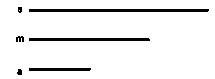
\includegraphics{../graphics/challenge1.pdf}
\]
\begin{enumerate}
\item Start with the given side.
\item Since the median hits our side at the center, bisect the given
  side.
\item Make a circle of radius equal to the length of the median
  centered at the bisector of the given side.
\item Construct a line parallel to our given line of distance equal to
  the length of the given altitude away.
\item Where the line and the circle intersect is the third point of
  our triangle. Connect the endpoints of the given side and the new
  point to get the triangle we want.
\end{enumerate}
\end{proof}


\begin{question} How can you construct a triangle given one angle $\alpha$, the 
length of an adjacent side $s$, and the altitude to that side $a$?
\end{question}

\begin{proof}[Follow-Along]
Use these and follow the directions below.
\[
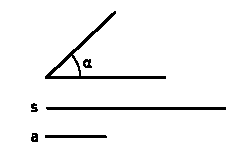
\includegraphics{../graphics/challenge2.pdf}
\]
\begin{enumerate}
\item Start with a line containing the side.
\item Put the angle at the end of the side.
\item Draw a parallel line to the side of the length of the altitude
  away.
\item Connect the angle to the parallel side. This is the third
  vertex. Connect the endpoints of the given side and the new point to
  get the triangle we want.
\end{enumerate}
\end{proof}


\begin{question} How can you construct a circle with a given radius tangent 
to two other circles?
\end{question}

\begin{proof}[Follow-Along]
Use these and follow the directions below.
\[
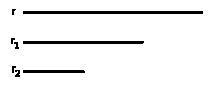
\includegraphics{../graphics/challenge3.pdf}
\]
\begin{enumerate}
\item Let $r$ be the given radius, and let $r_1$ and $r_2$ be the
  radii of the given circles.
\item Draw a circle of radius $r_1 + r$ around the center of the
  circle of radius $r_1$.
\item Draw a circle of radius $r_2 + r$ around the center of the
  circle of radius $r_2$.
\item Where the two circles drawn above intersect is the center of the
  desired circle.
\end{enumerate}
\end{proof}


\begin{question} 
Place two tacks in a wall. Insert a sheet of paper so that the edges
hit the tacks and the corner passes through the imaginary line between
the tacks. Mark where the corner of the piece of paper touches the
wall. Repeat this process, sliding the paper around. What curve do you
end up drawing?
\end{question}
\QM

\begin{question} How can you construct a triangle given an angle and the 
length of the opposite side?
\end{question}

\begin{proof}[Solution] 
We really can't solve this problem completely because the information
given doesn't uniquely determine a triangle. However, we can still say
something. Here is what we can do:
\begin{enumerate}
\item Put the known angle at one end of the line segment. Note in the
  picture below, it is at the left end of the line segment and it is
  opening downwards.
\item Construct the perpendicular bisector of the given segment.
\item See where the bisector in Step 2 intersects the perpendicular of
  the other leg of the angle drawn from the vertex of the angle.
\item Draw arc centered at the point found in Step 3 that
  touches the endpoints of the original segment.
\end{enumerate}
\[
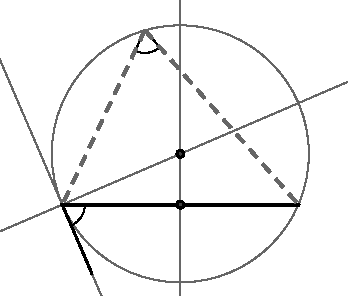
\includegraphics[scale=0.9]{../graphics/challenge4.pdf}
\]
Every point on the arc is a valid choice for the vertex of the
triangle.
\end{proof}

\begin{question} Why does the above method work?
\end{question}
\QM

\begin{question}\index{boat!lost at night} 
You are on a boat at night. You can see three lighthouses, and you
know their position on a map.  Also you know the angles of the light
rays between the lighthouses as measured from the boat.  How do you
figure out where you are?
\end{question}
\QM

\subsection{Problem Solving Strategies}

The harder constructions discussed in this section can be difficult to
do. There is no rote method to solve these problems, hence you must
rely on your brain. Here are some hints that you may find helpful:

\paragraph{Construct what you can.} 
You should start by constructing anything you can, even if you don't
see how it will help you with your final construction. In doing so you
are ``chipping away'' at the problem just as a rock-cutter chips away
at a large boulder. Here are some guidelines that may help when
constructing triangles:
\begin{enumerate}
\item If a side is given, then you should draw it.
\item If an angle is given and you know where to put it, draw it.
\item If an altitude of length $\l$ is given, then draw a line
  parallel to the side that the altitude is perpendicular to. This new
  line must be distance $\l$ from the side.
\item If a median is given, then bisect the segment it connects to and
  draw a circle centered around the bisector, whose radius is the
  length of the median.
\item If you are working on a figure, construct any ``mini-figures''
  inside the figure you are trying to construct. For example, many of
  the problems below ask you to construct a triangle. Some of these
  constructions have right-triangles inside of them, which are easier
  to construct than the final figure.
\end{enumerate}



\paragraph{Sketch what you are trying to find.} 
It is a good idea to try to sketch the figure that you are trying to
construct. Sketch it accurately and label all pertinent parts. If
there are special features in the figure, say two segments have the
same length or there is a right-angle, make a note of it on your
sketch. Also mark what is unknown in your sketch. We hope that doing
this will help organize your thoughts and get your ``brain juices''
flowing.\index{brain juices}

\begin{question} Why are the above strategies good?
\end{question}
\QM


\begin{problems}
\begin{enumerate}

%%% In Polya's book ``Mathematical Discovery'' he has some interesting
%%% notation for problems like the ones we give below. It may be good to
%%% use something like that in the future.

\item Construct a square. Explain the steps in your construction.

\item Construct a regular hexagon. Explain the steps in your construction.


\item Your friend Margy is building a clock. She needs to know how to align
the twelve numbers on her clock so that they are equally spaced on a
circle. Explain how to use a compass and straightedge construction to
help her out. Illustrate your answer with a construction and explain
the steps in your construction.

\item Construct a triangle given two sides of a triangle and the angle
  between them. Explain the steps in your construction.

\item State the SAS Theorem.

\item Construct a triangle given three sides of a triangle. Explain
  the steps in your construction.

\item State the SSS Theorem.


\item Construct a triangle given a side and two angles where one of
  the angles does not touch the given side. Explain the steps in your
  construction.

\item State the SAA Theorem.

\item Construct a triangle given a side between two given
  angles. Explain the steps in your construction.

\item State the ASA Theorem.

\item Explain why when given an isosceles triangle, that two
  of its angles have equal measure. Hint: Use the SAS Theorem.


\item Construct a figure showing that a triangle cannot always be
  uniquely determined when given an angle, a side adjacent to that
  angle, and the side opposite the angle. Explain the steps in your
  construction and explain how your figure shows what is
  desired. Explain what this says about the possibility of a SSA
  theorem.  Hint: Draw many pictures to help yourself out.

\item Give a construction showing that a triangle is uniquely
  determined if you are given a right-angle, a side touching that
  angle, and another side not touching the angle. Explain the steps in
  your construction and explain how your figure shows what is desired.

\item Construct a triangle given two adjacent sides of a triangle and
  a median to one of the given sides. Explain the steps in your
  construction.

\item Construct a triangle given two sides and the altitude to the
  third side. Explain the steps in your construction.

\item Construct a triangle given a side, the median to the side, and
  the angle opposite to the side. Explain the steps in your
  construction.

%\item Construct a triangle given two altitudes and an angle touching
%  one of them. Explain the steps in your construction. %% TANGENTS NEEDED


\item Construct a triangle given an altitude, and two angles not
  touching the altitude. Explain the steps in your construction.

\item Construct a triangle given the length of one side, the length of
  the the median to that side, and the length of the altitude of the
  opposite angle. Explain the steps in your construction.

\item Construct a triangle, given one angle, the length of an adjacent
  side and the altitude to that side. Explain the steps in your
  construction.

\item Construct a circle with a given radius tangent to two other
  given circles. Explain the steps in your construction.

\item Does a given angle and a given opposite side uniquely determine
  a triangle? Explain your answer.

\item You are on the bank of a river. There is a tree directly in
  front of you on the other side of the river. Directly left of you is
  a friend a known distance away. Your friend knows the angle starting
  with them, going to the tree, and ending with you. How wide is the
  river? Explain your work.

\item You are on a boat at night. You can see three lighthouses, and
  you know their position on a map.  Also you know the angles of the
  light rays from the lighthouses.  How do you figure out where you
  are? Explain your work.

\item Construct a triangle given an angle, the length of a side
  adjacent to the given angle, and the length of the angle's bisector
  to the opposite side. Explain the steps in your construction.

\item Construct a triangle given an angle, the length of the opposite
  side, and the length of the altitude of the given angle. Explain the
  steps in your construction.

\item Construct a triangle given one side, the length of the altitude
  of the opposite angle, and the radius of the circumcircle. Explain
  the steps in your construction.

\item Construct a triangle given one side, the length of the altitude
  of an adjacent angle, and the radius of the circumcircle. Explain
  the steps in your construction.

\item Construct a triangle given one side, the length of the median
  connecting that side to the opposite angle, and the radius of the
  circumcircle. Explain the steps in your construction.  

\item Construct a triangle given one angle and the lengths of the
  altitudes to the two other angles. Explain the steps in your
  construction.

\item Construct a circle with a given radius tangent to two given
  intersecting lines. Explain the steps in your construction.

\item Given a circle and a line, construct another circle of a given
  radius that is tangent to both the original circle and line. Explain
  the steps in your construction.

\item Construct a circle with three smaller circles of equal size
  inside such that each smaller circle is tangent to the other two and
  the larger outside circle. Explain the steps in your construction.

\end{enumerate}
\end{problems}
